\documentclass[twoside,french]{report}
\usepackage[francais]{babel}
\usepackage[T1]{fontenc}
\usepackage[utf8]{inputenc}
\usepackage[letterpaper]{geometry}
\usepackage{amsmath}
\usepackage{graphicx}

% For source code coloring and formatting
\usepackage{listings} 
\lstset{mathescape,basicstyle=\ttfamily}% Allow escaping to LaTeX inside $..$




\usepackage[pdftex,
      pdfauthor={Guillaume Legrain & Florian Martin},
      pdftitle={Projet Java A3P},
      colorlinks
      ]{hyperref}

\setlength{\topmargin}{-0.5in}
\setlength{\textheight}{9in}
\setlength{\oddsidemargin}{.125in}
\setlength{\textwidth}{6.25in}

%\setcounter{chapter}{1}

\begin{document}

\begin{titlepage}

\title{Projet Java A3P}
\date{\today}
\author{Guillaume Legrain \\
        Florian Martin \\
        Groupe 3J E3S}
\maketitle
%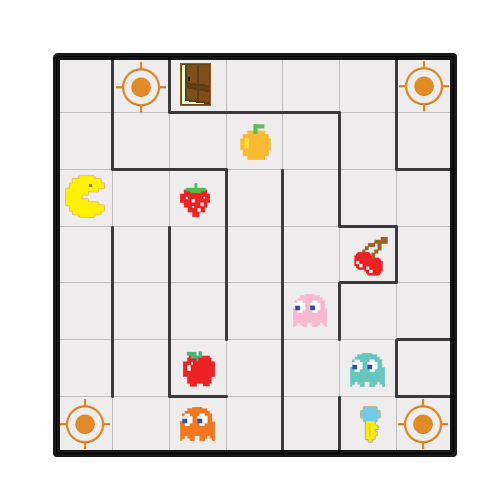
\includegraphics[scale=0.8]{graphics/Plan-Projet-1.png}
%\begin{abstract}
% Pac-Man dans un nouveau monde, sous un nouvel angle.\vspace{-2ex}
%\end{abstract}
\end{titlepage}

\tableofcontents

\chapter{Présentation du projet}
Vous êtes Pac-Man, perdu dans un étrange labyrinthe peuplé de fantômes. Vous voulez vous échapper.
Mais il faut trouver la clef de la sortie ainsi que des fruits pour affronter les fantômes qui en
bloquent l’accès.

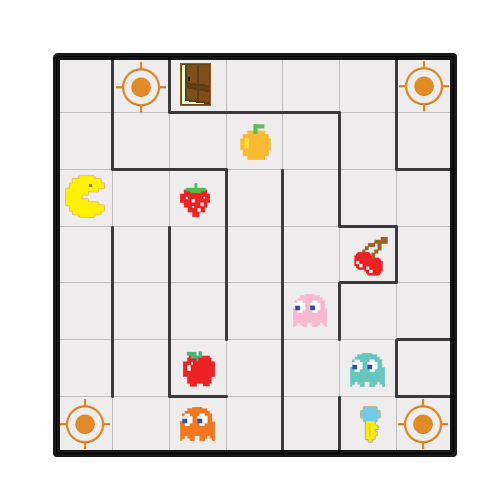
\includegraphics[scale=0.8]{graphics/Plan-Projet-1.png}

\section{Buts}
   \begin{itemize}
      \item But principal: trouver la clef pour pouvoir ouvrir la porte et sortir du labyrinthe.
      \item Les fantômes sont dangereux ! Il faut donc trouver et manger assez de fruits pour
      pouvoir les affronter.
      \item Pour aller plus vite, Pac-Man peut utiliser des téléporteurs. Mais attention, ils ne 
      sont pas toujours très fiable et peuvent parfois conduire à des pièces sans issues.
   \end{itemize}

\section{Idées ...}
Note: Tous ces points ne seront pas forcément implémentés vu que nous ne pouvons pas encore 
vraiment savoir ce qui est envisageable à notre niveau.
   \begin{itemize}
      \item Chaque case du labyrinthe sera en fait une "pièce" avec des sorties
      (Nord, Sud, Est, West)
      \item Le joueur pourra choisir parmi plusieurs labyrinthes ( peut être même en 
      créer lui-même, dans un fichier que le jeu va "parser" avant de démarrer). %Une première approche
      %sera d'essayer de charger le niveau enregistré au format JSON ou XML et de le parser. %avec 
      %\href{https://github.com/douglascrockford/JSON-java}{JSON-java} ou \href{https://code.google.com/p/google-gson/}{google-gson}
      %par exemple.
      \item EN PLUS de la console (avec le "prompt"), le joueur pourra se déplacer avec les 
      touches du clavier (Up, down, left, right).
      \item Le Pac-Man se déplace aussi, en temps réel sur l'écran.
      \item Dessiner le plan du labyrinthe en Java (ou autre si mieux ...) suivant sa description
      plutôt que d'afficher une ou des images statiques.
      \item Créer une carte évolutive qui se met a jour lors du passage dans une piece.
      \item Imposer un certain nombre de fruit pour vaincre un type de fantôme.
      \item Insérer une musique dans le jeu.
      \item Insérer des sons lors de la récupération d'objet (clé, fruit) ou l'appartion d'un fantôme
   \end{itemize}

\section{Organisation d'un plan}
   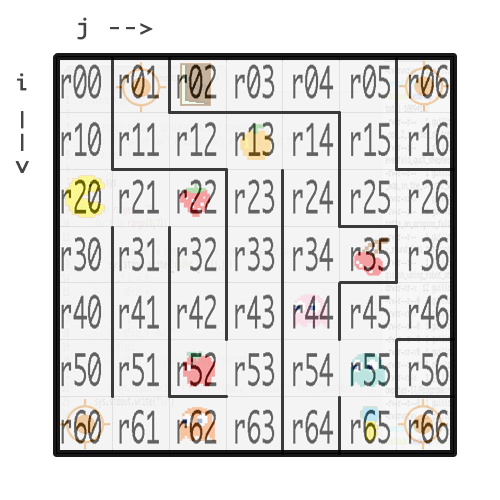
\includegraphics[scale=0.4]{graphics/Plan-Projet-1_numbered.png} \\
   Chaque "Room" est représentée par rij indiquant sa position sur le plan.
   Chaque "Room" possède des attributs indiquant la position de la case suivante ou un mur (avec un \lstinline|null| )



\chapter{Avancement des exercices}
\subsection*{Exercice 7.0 : }
Création de la page web

\subsection*{Exercice 7.1 : }
Découverte de zuul-bad

\subsubsection*{La classe Room}
Création de la première salle avec pour attributs la description de la salle et quatre sorties (Nord, Sud, Est, West)
\subsubsection*{La classe Command}
Création de la commande « go ». On doit déterminer dans un premier si un ou deux mots ont été tapés. Ensuite on doit vérifier si les commandes tapés sont valides d’où  l’introduction d’une fonction booléenne « isUnknown »
\subsubsection*{La classe Game}
\begin{itemize}
\item Création d’une méthode « createRooms » ayant pour but d’initialiser le jeux (les salles, les sorties, le lieu courant)
\item La procédure « goRoom » doit s’assurer de la présence d’un second mot (direction) et doit vérifier l’égalité de ce second mot avec une direction avec la fonction « equals ». Si les conditions sont réunis « goRoom » change la current room
\item On ajoute de nouvelles méthodes : 2 procédures renvoyant un message de bienvenue et un message d’aide. La première doit pouvoir faire appel à la current room et à ses différentes sorties. La seconde doit pouvoir renvoyer le nom de chaque commande disponible. On crée donc des procédure auxquelles on fera appel pour renvoyer ces informations et cela indépendamment du message écrit.
\item On crée une procédure « processCommand » renvoyant un booléen, capable d’appeler la bonne méthode en fonction de la commande passée en paramètre
\end{itemize}

\subsubsection*{Les classes CommandWords et Parser}
La classe CommandWords contient les mots de commande acceptés par le jeu\\
La classe Parser lie les commandes tapée au clavier, vérifie si la commande est valide et construit l’objet « Command » correspondant auquel on fera appel\\
V Jeu fonctionnel\\
On ajoute dans la classe Game un attribut aParser et une procédure « play» qui doit lire répétitivement les commandes tapé au clavier et les exécuter jusqu’à ce que l’on tape « quit ». On introduit une boucle while qui s’exécutera jusqu’à ce qu’une variable booléenne soit égal à vrai. Ce changement d’état aura lieu lorsque l’on tapera la commande « quit ».\\   

\subsection*{Exercice 7.1.1 : Thème}

\subsection*{Exercice 7.2.1 : La classe Scanner}

On crée un objet Scanner possédant le clavier en tant que paramètre. Les lignes de caractères tapés au clavier seront retranscrites dans une String.\\

\subsection*{Exercice 7.4 : Room}

On intègre dans le jeu les différentes salles qui compose notre scénario\\

\subsection*{Exercice 7.5 : printLocationInfo}

On ajoute une méthode affichant les informations de la current Room (nom pour l’instant)\\


\subsection*{Exercice 7.6 : getExit}

On ajoute une méthode renvoyant les sorties de la current Room

\subsection*{Exercice 7.7 : getExitString}

On modifie la méthode « printLocationInfo » pour qu’elle affiche aussi les sorties de la current Room. On fait appel pour cela à la méthode «  getExit »

\subsection*{Exercice 7.8 : HashMap, setExit}

On modifie la classe Room pour qu’elle possède un attribut aExit sous la forme d’une HashMap regroupant ainsi toutes les sorties. 

\subsection*{Exercice 7.9 : keySet}

\subsection*{Exercice 7.10 : getExitString CCM ?}

ToDo

\subsection*{Exercice 7.11 : getLongDescription}

ToDo

\subsection*{Exercice 7.14 :  look}
On ajoute une commande « look » faisant appel à la procédure  « getLongDesciption »  pour que le joueur puisse obtenir les informations de la current Room

\subsection*{Exercice 7.15 : eat}
On ajoute une commande « eat » qui pour l’instant ne renvoie qu’une String mais aura une interaction futur lorsque on ajoutera les Items

\subsection*{Exercice 7.16 : showAll, showCommand}
On ajoute une nouvelle méthode faisant appel à une boucle « for each » qui parcourt les commandes que l’on ajoute dans le jeu

\subsection*{Exercice 7.18 : getCommandList}
On ajoute une nouvelle méthode renvoyant les noms des commandes que l’on ajoute dans le jeu

\subsection*{Exercice 7.18.1 : comparaison à zuul-better}
ToDo

\subsection*{Exercice 7.18.2 : StringBuilder}
Le StringBuilder permet d’ajouter à une première String de nouveau charactères (ex : on ajoute la liste des commandes disponibles à la String « les actions que vous pouvez executer sont : » ) et ainsi de pouvoir une seul et unique String

\subsection*{Exercice 7.18.3 : recherche d’image}

\subsection*{Exercice 7.18.4 : titre du jeu}
TelePac pour faire référence aux téléporteurs et à Pac-Man tout en conservant un nom court et accrocheur

\subsection*{Exercice 7.18.5 : HashMap Rooms}
On créé une Hashmap contenant toutes les Room ce qui facilite l’organisation vu que le jeu contient 49 rooms

\subsection*{Exercice 7.18.6 : zuul-with-image}
On ajoute des images au jeu
\subsection*{Exercice 7.18.8 :} 
On ajoute des méthodes nécessitant un keyListenner afin de créer des boutons appelant les méthodes « quit », « look », …
\subsection*{Exercice 7.20 : Item}
On ajoute un objet Item a une Room avec pour attribut son nom et un poids 

\subsection*{Exercice 7.21 : Item description}

Les informations concernant les items doivent être stockés dans un premier temps au même endroit que celle de la Room puisque ToDo












\subsection*{Exercise 7.40:}

We have to add LOOK("look") to CommandWord and implement a action in Game.processCommand

\subsection*{Exercise 7.41:}

If we change the word associated with the help command in CommandWord, this change automatically reflected in the welcome text when you start the game.

\subsection*{Exercise 7.42:}

TODO: implement mvc

+ Added KeyListener to change room.

You can now go to another room using the keyboard's arrow keys.

\subsection*{Exercise 7.43: (Trap door)}

trap door player in room r06

TODO: empty previous room stack if trapdoor (the back command shouln't work)

TODO: show message

\subsection*{Exercise 7.44: (beamer)}

seems ok

\subsection*{Exercise 7.45: (locked door) (opt.)}

TODO: the player needs to find a key to open a locked door

NOTE:use heritage

\subsection*{Exercise 7.45.1: (update test files)}

TODO

\subsection*{Exercise 7.45.2: (update javadoc)}

TODO

\subsection*{Exercise 7.46: (TransporterRoom)}

+ Created a new TransporterRoom subclass from Room overriding getExit

Change r60, .. instantiation to TransporterRoom instead of Room

+ Added a getRooms method to the GameModel to get a Room HasMap

Converter the HashMap into a ArryList to select a value from a Random integer instead of a string description.

\subsection*{Exercise 7.46.1: (alea)}

TODO

\subsection*{Exercise 7.46.2:}

Beamer was already a item subclass

+ Created TrapRoom subclass (TODO: clear history when entering the room)

\subsection*{Exercise 7.53: (main)}

+ Added public static void main(String[] args) to instantiate a new game

\subsection*{Exercise 7.54: (without BlueJ)}

Launch the game using \"java Game\" in the game's directory
\end{document}
